\chapter{Cài đặt}
\label{Chapter4}
\setcounter{secnumdepth}{5}

\section{Độ đo đánh giá}

Để đánh giá hiệu suất phân đoạn của mô hình LViT và so sánh với các phương pháp tiên tiến khác (SOTA), báo cáo này sử dụng hai độ đo chính: \textbf{chỉ số Dice (Dice score)} và \textbf{mIoU (mean Intersection over Union)}.

\begin{itemize}
    \item \textbf{Chỉ số Dice (Dice score):} Đây là độ đo đánh giá mức độ trùng khớp giữa mặt nạ phân đoạn do mô hình dự đoán và mặt nạ nhãn chuẩn. Giá trị Dice càng cao cho thấy kết quả phân đoạn càng gần với nhãn chuẩn. Chỉ số này có mối liên hệ trực tiếp với hàm mất mát Dice, thường được biểu diễn dưới dạng $Dice = 1 - L_{Dice}$.

    \[
        Dice = \sum_{i=1}^{N} \sum_{j=1}^{C} \frac{1}{NC} \cdot \frac{2 | p_{ij} \cap y_{ij}|}{(|p_{ij}| + |y_{ij}|)}
    \]

    \item \textbf{mIoU (mean Intersection over Union):} Độ đo này tính tỷ lệ giữa phần giao nhau và phần hợp của vùng dự đoán so với vùng nhãn chuẩn, sau đó lấy trung bình trên các lớp cần phân đoạn. mIoU càng cao cho thấy vùng dự đoán càng khớp với vùng tổn thương thực tế.

    \[
        mIoU = \sum_{i=1}^{N} \sum_{j=1}^{C} \frac{1}{NC} \cdot \frac{|p_{ij} \cap y_{ij}|}{| p_{ij} \cup y_{ij}|}
    \]
\end{itemize}

Trong đó:
\begin{itemize}
    \item \textbf{$N$}: Tổng số điểm ảnh.
    \item \textbf{$C$}: Số lớp phân đoạn. Trong báo cáo này, $C$ được thiết lập bằng 1.
    \item \textbf{$p_{ij}$}: Xác suất mô hình dự đoán điểm ảnh $i$ thuộc về lớp $j$.
    \item \textbf{$y_{ij}$}: Nhãn chuẩn của điểm ảnh, có giá trị bằng 1 nếu điểm ảnh $i$ thuộc về lớp $j$ và bằng 0 trong trường hợp ngược lại.
\end{itemize}

\section{Môi trường thử nghiệm}

Thử nghiệm được thực hiện trên nền tảng Kaggle với cấu hình GPU T4 x2. Đây là môi trường phù hợp cho quá trình huấn luyện mô hình học sâu ở quy mô vừa, đặc biệt với các mô hình phân đoạn ảnh y khoa có kết hợp nhánh CNN và nhánh Transformer như LViT. Việc sử dụng GPU giúp tăng tốc đáng kể các phép tính ma trận, lan truyền tiến và lan truyền ngược trong quá trình tối ưu tham số.

Mô hình được huấn luyện riêng biệt trên hai tập dữ liệu QaTa-COV19-v2 và MosMedData+. Tập ESO-CT đã được đề cập trong phần phương pháp; tuy nhiên, tại thời điểm thực hiện báo cáo này, bộ dữ liệu này chưa được công bố công khai nên không thể truy cập để tiến hành thử nghiệm. Cách huấn luyện riêng từng tập dữ liệu giúp đánh giá khả năng học biểu diễn của LViT trên từng loại ảnh y khoa cụ thể, bao gồm ảnh X-ray ngực và ảnh CT phổi. Hai tập dữ liệu này đều có mặt nạ phân đoạn và ghi chú y khoa đi kèm, do đó phù hợp với mục tiêu đánh giá mô hình phân đoạn đa phương thức dựa trên cả thông tin ảnh và văn bản.

% Một điểm cần chú ý là định dạng chia sẻ của bộ dữ liệu MosMedData+ có sự thay đổi theo thời gian. Tại thời điểm các thử nghiệm trong báo cáo này được thực hiện, dữ liệu được cung cấp dưới dạng tệp nén .zip, bên trong bao gồm các ảnh đầu vào và phần chú thích tương ứng ở dạng file .csv. Cấu trúc này cho phép quá trình tiền xử lý được thực hiện theo hướng đọc trực tiếp từng ảnh, ánh xạ với thông tin chú thích trong bảng .csv, sau đó chuyển đổi về định dạng tensor phù hợp với mô hình.

% Tuy nhiên, khi báo cáo được hoàn thành, bộ dữ liệu MosMedData+ đã được chia sẻ lại ở định dạng .nii.gz. Đây là định dạng thường được sử dụng cho dữ liệu ảnh y khoa dạng thể tích, đặc biệt là ảnh CT. Sự thay đổi này không làm thay đổi mục tiêu đánh giá của thí nghiệm, nhưng có ảnh hưởng đến quy trình đọc dữ liệu và tiền xử lý nếu muốn tái lập kết quả ở thời điểm sau. Cụ thể, người tái lập cần kiểm tra lại cấu trúc dữ liệu hiện có, cách lưu trữ ảnh và annotation, cũng như bước chuyển đổi từ dữ liệu thể tích sang lát cắt hai chiều trước khi đưa vào mô hình LViT. Vì vậy, báo cáo ghi nhận rõ định dạng dữ liệu được sử dụng tại thời điểm thực nghiệm để tránh nhầm lẫn giữa kết quả huấn luyện trong báo cáo và phiên bản dữ liệu được công bố sau này.

% Vì thế báo cáo sẽ thay thế bằng dữ liệu MoNuSeg. https://monuseg.grand-challenge.org/Data/

Trước khi đưa vào mô hình, tất cả ảnh đầu vào được thay đổi kích thước về $224 \times 224$. Đây là kích thước đầu vào phổ biến của Vision Transformer, đặc biệt trong các mô hình tiền huấn luyện trên ImageNet. Việc sử dụng cùng kích thước này giúp đảm bảo sự tương thích với cơ chế chia ảnh thành các patch và với vector mã hoá vị trí trong nhánh Transformer. Ngoài ra, việc chuẩn hoá kích thước ảnh cũng giúp các batch có cùng kích thước tensor, giảm độ phức tạp khi huấn luyện và tạo điều kiện so sánh công bằng giữa các tập dữ liệu.

Các siêu tham số được lựa chọn theo hướng cân bằng giữa chất lượng học và giới hạn tài nguyên của môi trường Kaggle. Do ảnh y khoa và mặt nạ phân đoạn yêu cầu lưu trữ nhiều bản đồ đặc trưng trung gian, batch size được đặt nhỏ để tránh vượt quá bộ nhớ GPU. Learning rate được chọn ở mức tương đối nhỏ nhằm giúp quá trình tối ưu ổn định hơn, đặc biệt khi mô hình kết hợp nhiều thành phần mất mát khác nhau. Cấu hình hyperparameter được thiết lập như sau:

\begin{table}[H]
    \centering
    \begin{tabular}{lcccc}
    \hline
    \multirow{2}{*}{} & \multicolumn{2}{c}{\textbf{QaTa-COV19-v2}} & \multicolumn{2}{c}{\textbf{MosMedData+}} \\
    \cline{2-5}
    & Supervised & Semi-supervised & Supervised & Semi-supervised \\
    \hline
    \textbf{Optimizer} & \multicolumn{4}{c}{Adam} \\
    \textbf{Tỉ lệ nhãn} & 100\% & 25\% & 100\% & 25\% \\
    \textbf{Batch size} & 24 & 16 & 24 & 16 \\
    \textbf{Learning rate} & \multicolumn{2}{c}{0.0003} & \multicolumn{2}{c}{0.001} \\
    \textbf{Scheduler} & \multicolumn{4}{c}{Cosine Annealing Restarts} \\
    \textbf{Epochs} & \multicolumn{4}{c}{100} \\
    \hline
    \end{tabular}
\end{table}

\section{Chú thích mã nguồn}
Cấu trúc mã nguồn mô hình LViT được tổ chức như sau:

\dirtree{%
    .1 src/.
        .2 datasets/.
            .3 Covid19/.
            % .3 MoNuSeg/.
            .3 MosMedDataPlus/.
        .2 nets/.
            .3 LViT.py.
            .3 pixlevel.py.
            .3 textlevel.py.
            .3 UNet.py.
            .3 Vit.py.
        .2 Config.py.
        .2 Load\_Dataset.py.
        .2 requirements.txt.
        .2 test\_model.py.
        .2 train\_model.py.
        .2 Train\_one\_epoch.py.
        .2 utils.py.
}

Do môi trường thử nghiệm trong báo cáo này khác với môi trường thực thi được sử dụng trong công trình gốc, một số thành phần mã nguồn cần được điều chỉnh để có thể chạy ổn định trên nền tảng hiện tại. Cụ thể, báo cáo vẫn giữ lại các thư viện Python và cấu trúc cài đặt chính liên quan đến LViT, nhưng có rà soát và chỉnh sửa một số đoạn mã nhằm bảo đảm tương thích với phiên bản mới hơn của các thư viện học sâu, thư viện xử lý ảnh và các hàm hỗ trợ đọc dữ liệu.

Các thay đổi này chủ yếu tập trung vào những phần có khả năng bị ảnh hưởng bởi sự khác biệt phiên bản, chẳng hạn như cú pháp gọi hàm, xử lý tensor, định dạng dữ liệu đầu vào, quản lý bộ nhớ. Mục tiêu của các chỉnh sửa là giữ nguyên ý tưởng và luồng xử lý chính của mô hình LViT, đồng thời giúp mã nguồn có thể thực thi được trong môi trường Kaggle và với cấu trúc dữ liệu được sử dụng trong báo cáo này.

Những chỉnh sửa này không nhằm thay đổi bản chất kiến trúc mô hình hay phương pháp huấn luyện được trình bày trong các chương trước. Thay vào đó, chúng đóng vai trò tái lập thí nghiệm trong điều kiện phần mềm và dữ liệu hiện có. Danh sách thay đổi cụ thể, bao gồm các file được chỉnh sửa và lý do chỉnh sửa, cách chạy mã nguồn được trình bày chi tiết trong file README đính kèm trong thư mục mã nguồn.

\section{Cài đặt thực tế}
Các sơ đồ ở phần phương pháp cung cấp cái nhìn tổng quan về luồng xử lý của mô hình LViT, trong đó nhấn mạnh sự kết hợp giữa nhánh CNN, nhánh ViT và đặc trưng văn bản. Tuy nhiên, khi chuyển từ mô tả phương pháp sang cài đặt thực tế, một số thao tác cần được điều chỉnh để phù hợp với cách biểu diễn tensor trong các thư viện học máy. Ví dụ, các phép cộng, phép nối đặc trưng hoặc truyền dữ liệu giữa hai nhánh chỉ có thể thực hiện khi các tensor có cùng kích thước không gian, cùng số chiều hoặc đã được chiếu về cùng miền biểu diễn. Vì vậy, kiến trúc trong cài đặt có một số khác biệt so với sơ đồ khái niệm, dù vẫn giữ nguyên ý tưởng chính của mô hình.

Trong quá trình cài đặt, mỗi ảnh đầu vào được biểu diễn dưới dạng tensor bốn chiều gồm batch size, số kênh, chiều cao và chiều rộng. Các đặc trưng trung gian sinh ra từ nhánh CNN thường giữ cấu trúc không gian hai chiều, trong khi đặc trưng ở nhánh ViT cần được chuyển thành chuỗi token thông qua thao tác chia patch và làm phẳng. Do hai kiểu biểu diễn này khác nhau, mô hình cần thêm các bước biến đổi như reshape, transpose, projection, upsampling hoặc downsampling để bảo đảm dữ liệu có thể được kết hợp đúng cách. Những bước này không luôn được thể hiện đầy đủ trong sơ đồ phương pháp, nhưng lại rất quan trọng trong cài đặt thực tế.

\begin{figure}[H]
    \centering
    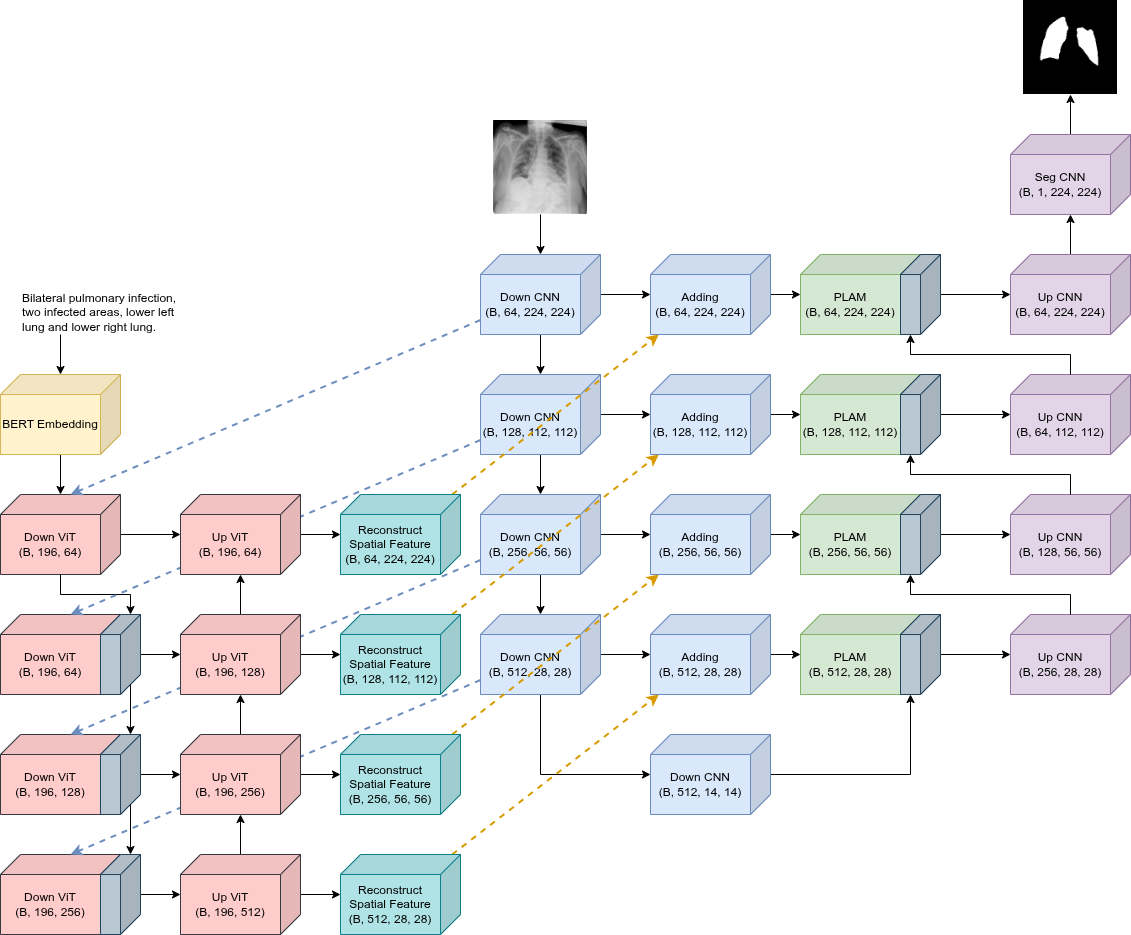
\includegraphics[width=0.7\linewidth]{images/implementation.png}
    \caption{Minh họa kiến trúc LViT trong cài đặt.}
\end{figure}

Bên cạnh việc mô tả các thành phần chính của mô hình, hình trên còn thể hiện kích thước dữ liệu được xử lý qua từng bước. Việc ghi rõ kích thước tensor giúp kiểm tra tính hợp lệ của kiến trúc trong quá trình cài đặt, đặc biệt tại các vị trí giao nhau giữa nhánh CNN và nhánh ViT. Nếu kích thước tensor không khớp, các phép toán như cộng phần dư, nối đặc trưng hoặc truyền qua khối tích chập sẽ không thể thực hiện. Do đó, sơ đồ cài đặt đóng vai trò như một bản kiểm tra luồng dữ liệu, giúp bảo đảm rằng đầu ra của mỗi khối có thể trở thành đầu vào hợp lệ cho khối tiếp theo.

Một ví dụ quan trọng là các khối nối đặc trưng được minh họa trong hình dưới đây:
\begin{figure}[H]
    \centering
    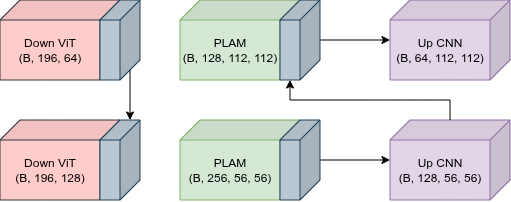
\includegraphics[width=0.7\linewidth]{images/concat.png}
    \caption{Phép nối dữ liệu theo chiều kênh.}
\end{figure}

Các khối màu xám thể hiện phép nối đặc trưng, trong đó nhiều tensor từ các nhánh khác nhau được ghép lại theo chiều kênh. Phép nối này làm tăng số kênh của dữ liệu, cho phép mô hình giữ lại đồng thời thông tin cục bộ từ CNN và thông tin ngữ nghĩa/toàn cục từ ViT. Tuy nhiên, trước khi nối, các tensor phải có cùng kích thước không gian. Vì vậy, tại những khối có đầu vào không tương đồng về chiều cao hoặc chiều rộng, cài đặt thực tế cần thực hiện thao tác tăng hoặc giảm kích thước.


\section{Kết quả thử nghiệm}

Kết quả thử nghiệm được tổng hợp từ quá trình huấn luyện, kiểm định và kiểm thử mô hình LViT trên hai tập dữ liệu QaTa-COV19-v2 và MosMedData+. Với mỗi tập dữ liệu, báo cáo xem xét hai cấu hình: huấn luyện có giám sát hoàn toàn (supervised) và huấn luyện bán giám sát (semi-supervised). Trong cấu hình bán giám sát, một phần dữ liệu được xem như không có nhãn bằng cách bỏ qua mặt nạ gốc trong quá trình huấn luyện, từ đó mô phỏng bối cảnh dữ liệu y khoa thiếu chú thích pixel.

\begin{figure}[H]
    \centering
    \setlength{\tabcolsep}{2pt}
    \begin{tabular}{cccccccc}
        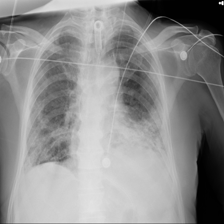
\includegraphics[width=0.115\linewidth]{comparison/sub-S08047_ses-E16280_run-1_bp-chest_vp-ap_dx.png} &
        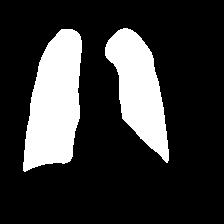
\includegraphics[width=0.115\linewidth]{comparison/sub-S08047_ses-E16280_run-1_bp-chest_vp-ap_dx.png_lab.jpg} &
        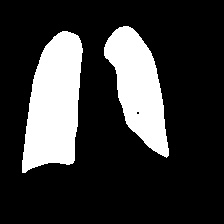
\includegraphics[width=0.115\linewidth]{comparison/sub-S08047_ses-E16280_run-1_bp-chest_vp-ap_dx.png_predictSupervisedLViT.jpg} &
        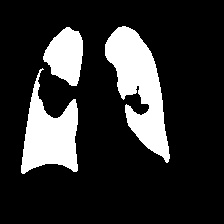
\includegraphics[width=0.115\linewidth]{comparison/sub-S08047_ses-E16280_run-1_bp-chest_vp-ap_dx.png_predictSemiLViT.jpg} &
        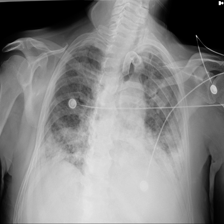
\includegraphics[width=0.115\linewidth]{comparison/sub-S08047_ses-E16628_run-1_bp-chest_vp-ap_dx.png} &
        
\includegraphics[width=0.115\linewidth]{comparison/sub-S08047_ses-E16628_run-1_bp-chest_vp-ap_dx.png_lab.jpg} &
        
\includegraphics[width=0.115\linewidth]{comparison/sub-S08047_ses-E16628_run-1_bp-chest_vp-ap_dx.png_predictSupervisedLViT.jpg} &
        
\includegraphics[width=0.115\linewidth]{comparison/sub-S08047_ses-E16628_run-1_bp-chest_vp-ap_dx.png_predictSemiLViT.jpg} \\
        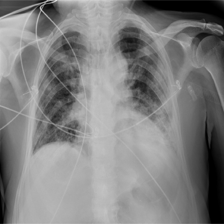
\includegraphics[width=0.115\linewidth]{comparison/sub-S08047_ses-E16837_run-1_bp-chest_cr.png} &
        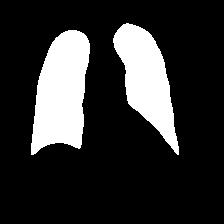
\includegraphics[width=0.115\linewidth]{comparison/sub-S08047_ses-E16837_run-1_bp-chest_cr.png_lab.jpg} &
        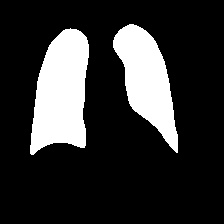
\includegraphics[width=0.115\linewidth]{comparison/sub-S08047_ses-E16837_run-1_bp-chest_cr.png_predictSupervisedLViT.jpg} &
        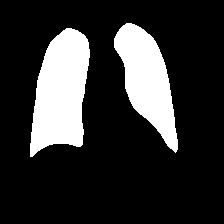
\includegraphics[width=0.115\linewidth]{comparison/sub-S08047_ses-E16837_run-1_bp-chest_cr.png_predictSemiLViT.jpg} &
        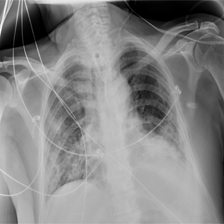
\includegraphics[width=0.115\linewidth]{comparison/sub-S08047_ses-E17130_run-1_bp-chest_cr.png} &
        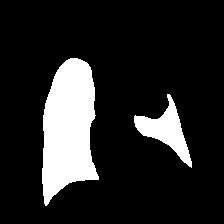
\includegraphics[width=0.115\linewidth]{comparison/sub-S08047_ses-E17130_run-1_bp-chest_cr.png_lab.jpg} &
        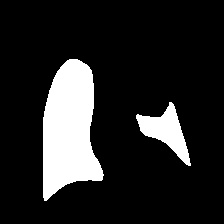
\includegraphics[width=0.115\linewidth]{comparison/sub-S08047_ses-E17130_run-1_bp-chest_cr.png_predictSupervisedLViT.jpg} &
        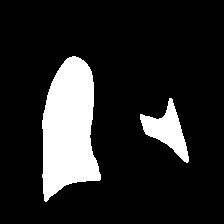
\includegraphics[width=0.115\linewidth]{comparison/sub-S08047_ses-E17130_run-1_bp-chest_cr.png_predictSemiLViT.jpg} \\
    \end{tabular}
    \caption{So sánh trực quan dự đoán trên QaTa-COV19, thứ tự từ trái sang phải là ảnh gốc, ground truth, mask supervised và mask semi-supervised.}
\end{figure}

\begin{figure}[H]
    \centering
    \setlength{\tabcolsep}{2pt}
    \begin{tabular}{cccccccc}
        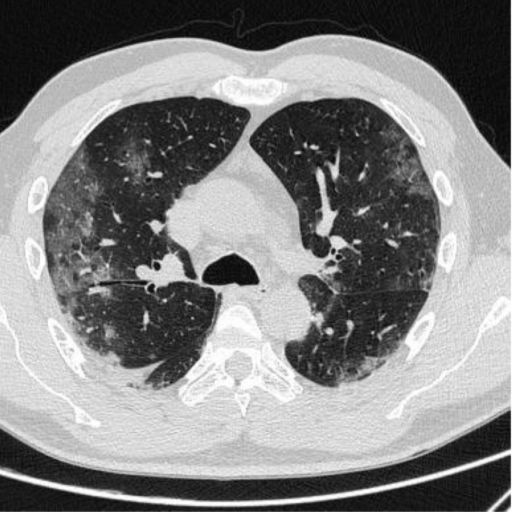
\includegraphics[width=0.115\linewidth]{comparison2/bjorke_81.png} &
        
\includegraphics[width=0.115\linewidth]{comparison2/bjorke_81.png_lab.jpg} &
        
\includegraphics[width=0.115\linewidth]{comparison2/bjorke_81.png_predictSupervisedLViT.jpg} &
        
\includegraphics[width=0.115\linewidth]{comparison2/bjorke_81.png_predictSemiLViT.jpg} &
        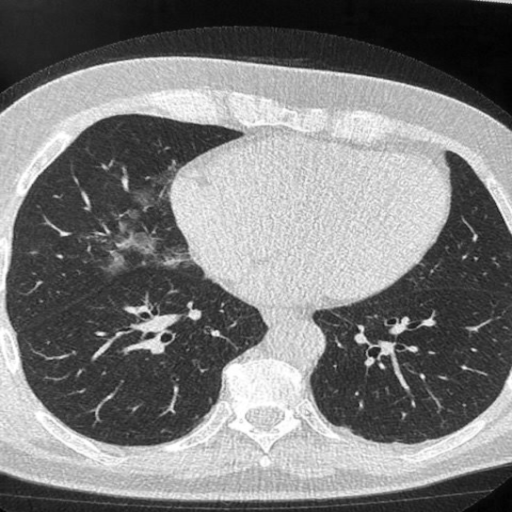
\includegraphics[width=0.115\linewidth]{comparison2/bjorke_82.png} &
        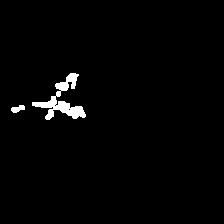
\includegraphics[width=0.115\linewidth]{comparison2/bjorke_82.png_lab.jpg} &
        
\includegraphics[width=0.115\linewidth]{comparison2/bjorke_82.png_predictSupervisedLViT.jpg} &
        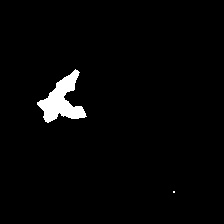
\includegraphics[width=0.115\linewidth]{comparison2/bjorke_82.png_predictSemiLViT.jpg} \\
        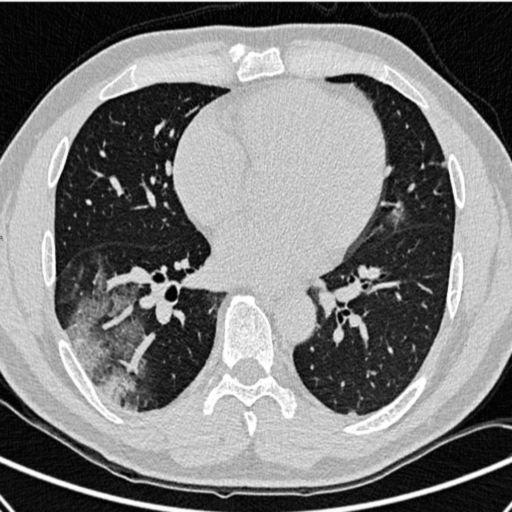
\includegraphics[width=0.115\linewidth]{comparison2/bjorke_83.png} &
        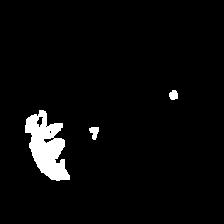
\includegraphics[width=0.115\linewidth]{comparison2/bjorke_83.png_lab.jpg} &
        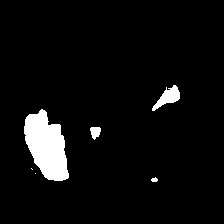
\includegraphics[width=0.115\linewidth]{comparison2/bjorke_83.png_predictSupervisedLViT.jpg} &
        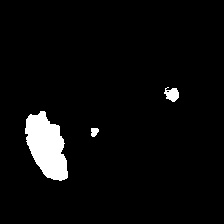
\includegraphics[width=0.115\linewidth]{comparison2/bjorke_83.png_predictSemiLViT.jpg} &
        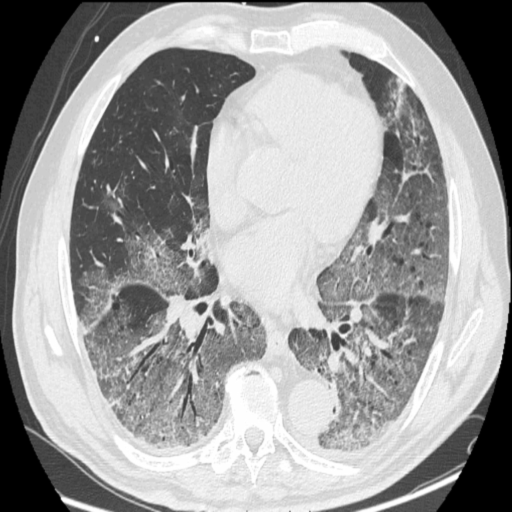
\includegraphics[width=0.115\linewidth]{comparison2/bjorke_9.png} &
        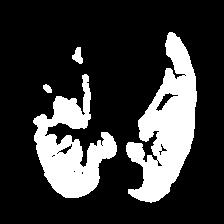
\includegraphics[width=0.115\linewidth]{comparison2/bjorke_9.png_lab.jpg} &
        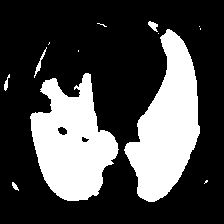
\includegraphics[width=0.115\linewidth]{comparison2/bjorke_9.png_predictSupervisedLViT.jpg} &
        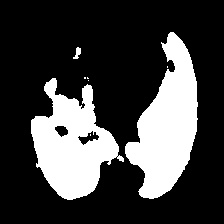
\includegraphics[width=0.115\linewidth]{comparison2/bjorke_9.png_predictSemiLViT.jpg} \\
    \end{tabular}
    \caption{So sánh trực quan dự đoán trên MosMedData+, thứ tự trong mỗi nhóm là ảnh gốc, ground truth, mask supervised và mask semi-supervised.}
\end{figure}

\begin{table}[H]
    \centering
    \caption{Kết quả huấn luyện, kiểm định và kiểm thử của LViT trên các cấu hình thực nghiệm}
    \resizebox{\linewidth}{!}{%
    \begin{tabular}{lccccc}
    \hline
    \textbf{Dữ liệu} & \textbf{Cấu hình} & \textbf{Train Dice} & \textbf{Val Dice} & \textbf{Test Dice} & \textbf{Test IoU} \\
    \hline
    Covid19 & Supervised & 86.32 & 79.44 & 81.27 & 72.46 \\
    Covid19 & Semi-supervised & 85.91 & 75.28 & 76.72 & 66.93 \\
    MosMedData+ & Supervised & 79.73 & 67.20 & 13.39 & 11.00 \\
    MosMedData+ & Semi-supervised & 78.79 & 63.86 & 12.92 & 10.44 \\
    \hline
    \end{tabular}%
    }
\end{table}

Trên tập Covid19, mô hình đạt kết quả tương đối ổn định. Ở cấu hình supervised, Test Dice đạt 81.27\% và Test IoU đạt 72.46\%. Đây là kết quả phù hợp với xu hướng quan sát được trong quá trình huấn luyện, vì Train Dice đạt 86.32\% và Val Dice đạt 79.44\%, cho thấy khoảng cách giữa huấn luyện, kiểm định và kiểm thử không quá lớn. Khi chuyển sang cấu hình semi-supervised, Test Dice giảm còn 76.72\% và Test IoU giảm còn 66.93\%. Mức giảm này là hợp lý vì mô hình không còn được sử dụng đầy đủ nhãn thật trong quá trình huấn luyện, trong khi phần sinh nhãn giả trong mã nguồn tái lập không hoàn toàn tương đương với một quy trình bán giám sát hoàn chỉnh trong công trình gốc.

Trên tập MosMedData+, kết quả có sự khác biệt rõ rệt giữa train/validation và test. Ở cấu hình supervised, Train Dice đạt 79.73\% và Val Dice đạt 67.20\%, nhưng Test Dice chỉ đạt 13.39\% và Test IoU đạt 11.00\%. Cấu hình semi-supervised cũng cho xu hướng tương tự, với Train Dice đạt 78.79\%, Val Dice đạt 63.86\%, nhưng Test Dice chỉ đạt 12.92\% và Test IoU đạt 10.44\%. Điều này cho thấy mô hình có học được đặc trưng trên tập huấn luyện, nhưng khả năng tổng quát hóa sang tập kiểm thử của MosMedData+ chưa tốt.

Nguyên nhân của sự khác biệt này đến từ nhiều yếu tố. Thứ nhất, MosMedData+ là dữ liệu CT phổi, có đặc điểm hình ảnh khác với ảnh X-ray trong Covid19. Dữ liệu CT có cấu trúc lát cắt, độ tương phản, phân bố cường độ và vùng tổn thương phức tạp hơn, nên quá trình tiền xử lý và chuẩn hóa dữ liệu ảnh hưởng mạnh đến chất lượng dự đoán. Thứ hai, phiên bản dữ liệu MosMedData+ được sử dụng trong quá trình tái lập có sự khác biệt về cách tổ chức và định dạng so với dữ liệu được mô tả trong công trình gốc, làm tăng nguy cơ sai khác trong bước đọc ảnh, ánh xạ mặt nạ và chia tập train/validation/test. Thứ ba, do giới hạn thời gian huấn luyện miễn phí trên Kaggle, mô hình chỉ được huấn luyện trong số epoch cố định, trong khi công trình gốc sử dụng cơ chế early stopping và không trình bày rõ số epoch thực tế trước khi dừng. Vì vậy, mô hình trong báo cáo có thể chưa đạt trạng thái hội tụ tốt nhất, đặc biệt trên MosMedData+.

Ngoài ra, trong mã nguồn được công bố của bài báo chính thức, phần học bán giám sát không được cài đặt đầy đủ, do đó báo cáo phải chỉnh sửa mã nguồn để có thể thử nghiệm cấu hình này. Về mặt dữ liệu, dữ liệu không nhãn được tạo ra bằng cách lấy 75\% dữ liệu gốc và bỏ qua phần nhãn đính kèm. Cách mô phỏng này giúp kiểm tra ý tưởng học bán giám sát, nhưng vẫn có khoảng cách so với một thiết lập bán giám sát hoàn chỉnh, nơi dữ liệu không nhãn thật sự có thể có phân bố khác và cần cơ chế kiểm soát chất lượng nhãn giả chặt chẽ hơn.

\begin{table}[H]
    \centering
    \caption{Kết quả so sánh LViT thử nghiệm với LViT công bố và các phương pháp SOTA}
    \resizebox{\linewidth}{!}{%
    \begin{tabular}{lcccccc}
    \hline
    \multirow{2}{*}{\textbf{Phương pháp}} & \multirow{2}{*}{\textbf{Văn bản}} & \multirow{2}{*}{\textbf{Tỉ lệ nhãn}} & \multicolumn{2}{c}{\textbf{QaTa-COV19}} & \multicolumn{2}{c}{\textbf{MosMedData+}} \\
    \cline{4-7}
    & & & Dice (\%) & mIoU (\%) & Dice (\%) & mIoU (\%) \\
    \hline
    \textbf{LViT-T-Exp} (1/4) & $\checkmark$ & 25\% & 76.72 & 66.93 & 12.92 & 10.44 \\
    \textbf{LViT-T-Exp} & $\checkmark$ & 100\% & 81.27 & 72.46 & 13.39 & 11.00 \\
    \hline
    LViT-TW (1/4) & $\times$ & 25\% & 79.08 & 69.42 & 70.65 & 58.07 \\
    LViT-TW (1/2) & $\times$ & 50\% & 80.35 & 70.74 & 71.89 & 59.63 \\
    LViT-TW & $\times$ & 100\% & 81.12 & 71.37 & 72.58 & 60.40 \\
    LViT-T (1/4) & $\checkmark$ & 25\% & 80.95 & 71.31 & 72.48 & 60.31 \\
    LViT-T (1/2) & $\checkmark$ & 50\% & 82.73 & 73.99 & 73.56 & 61.05 \\
    LViT-T & $\checkmark$ & 100\% & 83.66 & 75.11 & 74.57 & 61.33 \\
    \hline
    U-Net & $\times$ & 100\% & 79.02 & 69.46 & 64.60 & 50.73 \\
    UNet++ & $\times$ & 100\% & 79.62 & 70.25 & 71.75 & 58.39 \\
    nnUNet & $\times$ & 100\% & 80.42 & 70.81 & 72.59 & 60.36 \\
    \hline
    GLoRIA & $\times$ & 100\% & 79.94 & 70.68 & 72.42 & 60.18 \\
    LAVT & $\times$ & 100\% & 79.28 & 69.89 & 73.29 & 60.41 \\
    \hline
    \end{tabular}%
    }
\end{table}

Trong bảng trên, hậu tố \textbf{Exp} biểu thị các kết quả được tái lập trong báo cáo này, lấy từ quá trình huấn luyện và đánh giá thực nghiệm trên môi trường Kaggle. Ký hiệu \textbf{T} trong LViT-T chỉ phiên bản Tiny của LViT, trong đó mỗi khối DownViT sử dụng một lớp Transformer. Ký hiệu \textbf{W} trong LViT-TW biểu thị biến thể \textit{without text}, tức mô hình không sử dụng chú thích văn bản khi huấn luyện và suy luận. Các dòng không có hậu tố Exp là kết quả được công bố trong bảng so sánh gốc của công trình LViT. Vì vậy, bảng này không chỉ so sánh giữa các phương pháp, mà còn cho thấy khoảng cách giữa kết quả tái lập trong báo cáo và kết quả đã công bố.

Đối với dữ liệu Covid19, kết quả tái lập ở cấu hình 100\% nhãn đạt 81.27\% Dice và 72.46\% mIoU. Khi so với LViT-T công bố ở cùng tỉ lệ nhãn, mô hình tái lập thấp hơn 2.39 điểm Dice và 2.65 điểm mIoU. Khoảng cách này tương đối nhỏ so với các khác biệt thường gặp khi tái lập mô hình học sâu, đặc biệt khi môi trường phần mềm, cách chia dữ liệu và điều kiện dừng huấn luyện không hoàn toàn giống công trình gốc. Kết quả này cho thấy pipeline tái lập trên Covid19 đã giữ được phần lớn hiệu quả của LViT.

Ở cấu hình 25\% nhãn, LViT-T-Exp đạt 76.72\% Dice và 66.93\% mIoU, thấp hơn LViT-T công bố lần lượt 4.23 và 4.38 điểm. Mức giảm này lớn hơn cấu hình 100\% nhãn, cho thấy thiết lập bán giám sát trong báo cáo chưa tái hiện đầy đủ hiệu quả của cơ chế học bán giám sát trong công trình gốc. Nguyên nhân chính là phần học bán giám sát trong mã nguồn công bố không được cài đặt đầy đủ, nên báo cáo phải tự điều chỉnh để mô phỏng dữ liệu không nhãn bằng cách bỏ qua nhãn của một phần dữ liệu gốc.

Đối với MosMedData+, sự khác biệt giữa kết quả tái lập và kết quả công bố là rất lớn. Ở cấu hình 100\% nhãn, LViT-T công bố đạt 74.57\% Dice và 61.33\% mIoU, trong khi LViT-T-Exp chỉ đạt 13.39\% Dice và 11.00\% mIoU. Ở cấu hình 25\% nhãn, kết quả tái lập cũng chỉ đạt 12.92\% Dice và 10.44\% mIoU, thấp hơn rất nhiều so với 72.48\% Dice và 60.31\% mIoU của LViT-T công bố. Điều này cho thấy mô hình tái lập trên MosMedData+ chưa tổng quát tốt sang tập kiểm thử, mặc dù Train Dice và Val Dice vẫn đạt mức tương đối cao trong bảng kết quả phía trên.

Khi so sánh giữa LViT-T và LViT-TW trong kết quả công bố, có thể thấy thông tin văn bản giúp cải thiện hiệu suất ở cả hai bộ dữ liệu. Với 100\% nhãn, LViT-T tăng từ 81.12\% lên 83.66\% Dice trên QaTa-COV19 và từ 72.58\% lên 74.57\% Dice trên MosMedData+ so với LViT-TW. Điều này củng cố nhận định rằng chú thích văn bản đóng vai trò như tín hiệu ngữ nghĩa bổ sung, giúp mô hình định hướng vùng cần phân đoạn tốt hơn so với chỉ sử dụng đặc trưng ảnh.

Mặt khác, trong các kết quả công bố của LViT, cấu hình chỉ sử dụng 25\% dữ liệu có nhãn vẫn đạt Dice và mIoU tương đối ổn định so với nhiều phương pháp SOTA sử dụng toàn bộ nhãn. Điều này cho thấy cơ chế tạo nhãn giả EPI có vai trò quan trọng trong việc khai thác phần dữ liệu không nhãn: thay vì chỉ học từ số lượng mặt nạ thủ công bị giới hạn, mô hình có thể tận dụng dự đoán trung gian để bổ sung tín hiệu giám sát trong quá trình huấn luyện. Nhờ đó, không gian đặc trưng học được ít phụ thuộc hơn vào một tập nhãn nhỏ ban đầu và có khả năng bao quát tốt hơn các biến thiên về hình dạng, kích thước và vị trí tổn thương.

Tuy nhiên, kết quả tái lập trong báo cáo này cũng cho thấy hiệu quả của cấu hình 25\% nhãn phụ thuộc mạnh vào mức độ hoàn chỉnh của quy trình bán giám sát. Trên Covid19, LViT-T-Exp vẫn đạt kết quả chấp nhận được dù thấp hơn mô hình công bố, cho thấy ý tưởng tận dụng dữ liệu ít nhãn vẫn có giá trị trong điều kiện thực nghiệm hạn chế. Ngược lại, trên MosMedData+, kết quả thấp cho thấy cách mô phỏng dữ liệu không nhãn bằng việc bỏ qua nhãn gốc chưa đủ để tái hiện đầy đủ lợi ích của EPI, đặc biệt khi dữ liệu CT có cấu trúc lát cắt phức tạp, vùng tổn thương khó phân biệt và thời gian huấn luyện bị giới hạn. Vì vậy, EPI có tiềm năng giúp giảm chi phí chú thích dữ liệu y khoa, nhưng cần quy trình sinh, lọc và cập nhật nhãn giả chặt chẽ hơn để phát huy hiệu quả ổn định.